\documentclass[12pt]{article}

\usepackage[T1]{fontenc}
\usepackage[polish]{babel}
\usepackage[utf8]{inputenc}
\usepackage{lmodern}
\usepackage{graphicx}
\selectlanguage{polish}


\begin{document}

\title{Najpopularniejsze systemy liczbowe}
\author{Paweł Luszuk}
\date{\today}
\maketitle
\setcounter{tocdepth}{2} %shows all levels incl. paragraph
\begin{center}

\includegraphics[scale=0.25]{jpg3.jpg}
\end{center}

\newpage
\begin{flushleft}

\tableofcontents
\end{flushleft}


\newpage
\section{Wprowadzenie}
Ludzie, którzy na co dzień używają tylko systemu dziesiętnego do zapisu liczb czasem nie potrafią zrozumieć, jaka jest różnica pomiędzy systemem liczbowym a wartością liczby. System liczenia to sposób, w jaki zapisuje się liczby, a także algorytmy, dzięki którym z zapisu można odczytać wartość liczby. Poza tym system liczenia to także reguły, za pomocą, których można na liczbach zapisanych w konkretny sposób wykonywać działania.


\section{System dziesiętny}
\subsection{Definicja}
Najpowszechniej używanym sposobem przedstawiania liczb naturalnych jest system dziesiętny,gdzie na przykład zapis $$178$$ przedstawia liczbę składającą się z jednej setki siedmiu dziesiątek i ośmiu jedności.Możemy to zapisać w postaci $$178=1\cdot100+7\cdot10+8\cdot1$$ albo inaczej $$178=1\cdot10^2+7\cdot10^1+8\cdot10^0$$Tak więc w systemie dziesiętnym kolejne cyfry oznaczają współczynniki przy kolejnych potęgach liczby dziesięć, zaczynając od największej a kończąc na najmniejszej potędze.Mówimy, że liczba dziesięć jest podstawą lub bazą systemu dziesiętnego.
\subsection{Ogólny zapis}
 W systemie dziesiętnym używamy dziesięciu cyfr: $$0,1,2,3,4,5,6,7,8,9,0$$ a zapis $$d_rd_{r-1}...d_1d_0$$oznacza liczbę$$d_r\cdot10^r+d_{r-1}\cdot10^{r-1}+...+d_1\cdot10^1+d_0\cdot10^0$$

\newpage
\section{System binarny}
\subsection{Ogólny zapis}
W informatyce bardzo ważnym systemem liczbowym jest system binarny (dwójkowy),gdzie podstawą jest liczba 2 i gdzie mamy tylko dwie cyfry,1 i 0.Zapis$$d_rd_{r-1}...d_1d_0$$oznacza liczbę

$$\sum_{i=0}^{r} d_i\cdot2^i=d_r\cdot2^r+d_{r-1}\cdot2^{r-1}+...+d_1\cdot2^1+d_0\cdot2^0$$
\subsection{Porównanie z systemem dziesiętnym}
W poniższej tabeli przedstawiono siedemnaście kolejnych liczb w postaci dwójkowej i dziesiętnej
\\
\\
\\

{\centering
\begin{tabular}{|c|c|}
\hline
Dwójkowy&Dziesiętny\\ \hline
0&0\\
1&1\\
10&2\\
11&3\\
100&4\\
101&5\\
110&6\\
111&7\\
1000&8\\
1001&9\\
1010&10\\
1011&11\\
1100&12\\
1101&13\\
1110&14\\
1111&15\\
10000&16\\
\hline
\end{tabular}
\\}

\newpage

\subsection{Operacje arytmetyczne w systemie binarnym }
\begin{center}
$$Dodawanie\left\{
\begin{array}{ccc}
10101+111=11100\\
11+1=100\\


\end{array}
\right.$$

 

$$Odejmowanie\left\{
\begin{array}{ccc}
10101-111=1110\\
11-1=10\\


\end{array}
\right.$$


$$Mnożenie\left\{
\begin{array}{ccc}
10101\cdot111=10010011\\
11\cdot1=11\\


\end{array}
\right.$$

$$Dzielenie\left\{
\begin{array}{ccc}
10101:111=111\\
11:1=11\\


\end{array}
\right.$$

\end{center}

\begin{center}
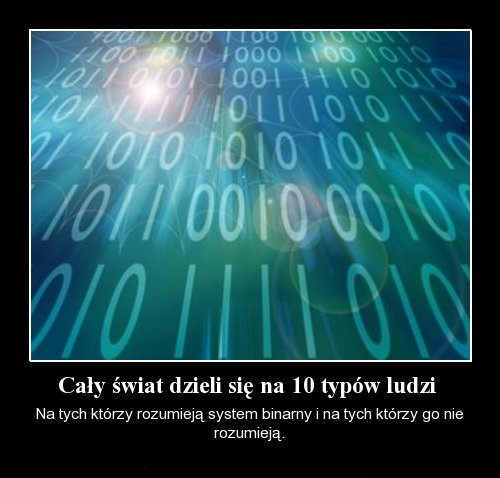
\includegraphics[scale=0.8]{jpg1.jpg}
\end{center}

\newpage
\section{System szesnastkowy}
\subsection{Definicja}
W informatyce używa się też systemu szesnastkowego, gdzie podstawą jest liczba 16.do systemu szesnastkowego potrzebujemy szesnastu cyfr.Zwykle używa się następujących ,,cyfr'':$$0,1,2,3,4,5,6,7,8,9,A,B,C,D,E,F$$ 
\subsection{Porównanie z pozostałymi systemami}
W poniższej tabeli zestawiono cyfry systemu szesnastkowego z odpowiadającymi im liczbami w systemie dwójkowym i dziesiętnym.
\\
\\
\\

{\centering
\begin{tabular}{|c|c|c|}
\hline
Szesnastkowy&Dwójkowy&Dziesiętny\\ \hline
0&0000&0\\
1&0001&1\\
2&0010&2\\
3&0011&3\\
4&0100&4\\
5&0101&5\\
6&0110&6\\
7&111&7\\
8&1000&8\\
9&1001&9\\
A&1010&10\\
B&1011&11\\
C&1100&12\\
D&1101&13\\
E&1110&14\\
F&1111&15\\

\hline
\end{tabular}
\\}

\begin{figure}[!ht]
	\centering
		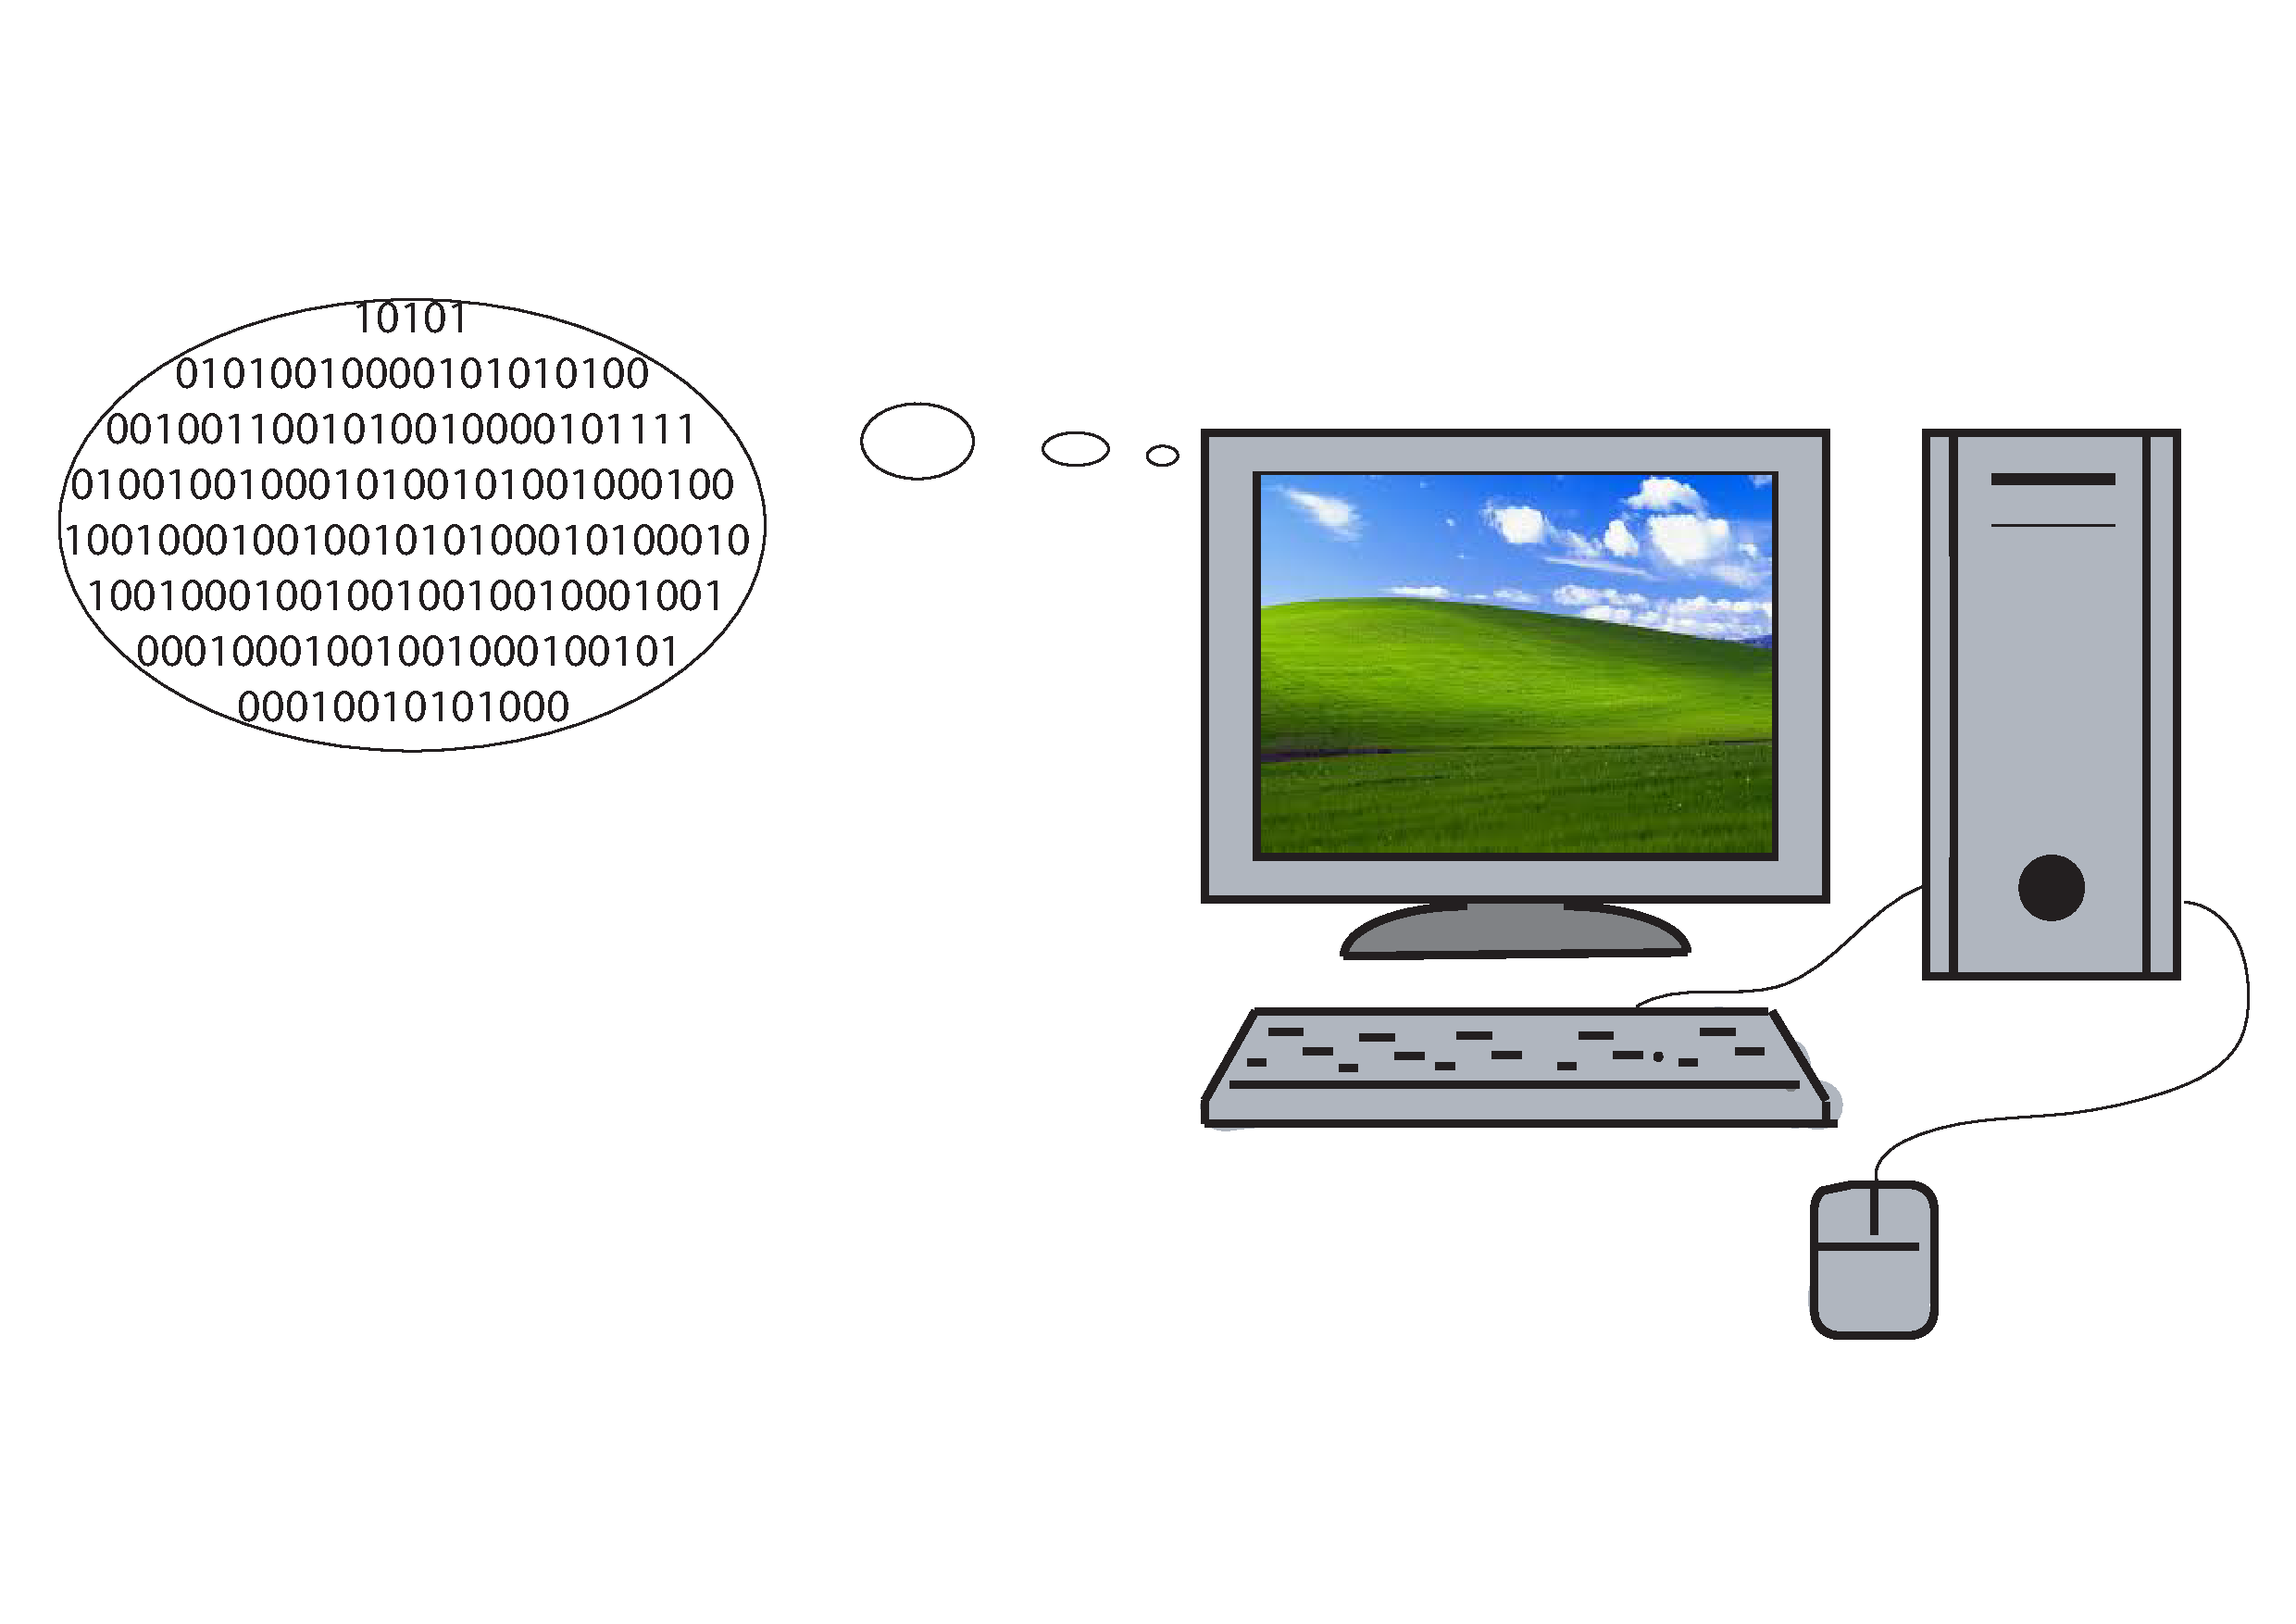
\includegraphics[scale=0.9,width=300pt]{computer.pdf}
	\caption{Komputer kontemplujący nad sensem istnienia w grafice wektorowej}
	
\end{figure}


\newpage
\section{Bibliografia}

\begin{thebibliography}{9}



\bibitem{knuthwebsite} 
A.Szpietowski, \textit{Matematyka dyskretna}, Wydawnictwo Uniwersytetu Gdańskiego,Gdańsk 2010.


\bibitem{knuthwebsite} 
Wikipedia
\\\texttt{www.wikipedia.pl}


\end{thebibliography}


\end{document}